



\section{Disponibilidade (\textit{Availability})}
Disponibilidade é a probabilidade de tempo de um sistema que está em condições de funcionar e pronto a responder a qualquer pedido de serviço a qualquer momento que lhe for pedido. Além de muitos objetivos a serem cumpridos este, \textit{availability}, deve ser visto como o mais prioritário porque um utilizador/empresa não gosta de ficar com um serviço indisponível.

Numa linguagem mais científica presente na \ac{EI} é usada a regra dos "9" para quantificar a disponibilidade média. No geral, o esperado numa empresa será atingir a meta dos cem por cento ou então "99,999" por cento na regra dos "9".

Existem fatores que comprometem a disponibilidade de uma rede como por exemplo a falha de energia elétrica, falha ou limites de conexão, quebra de algum componente de hardware ou algum ataque informático.


\section{Single Point of Failure}
Um \ac{SPOF} é uma parte de um sistema que, se falhar, interromperá o funcionamento de todo o sistema. \textit{SPOF's} são indesejáveis em qualquer sistema com o objetivo de alta disponibilidade ou fiabilidade.

\vspace{1cm}

\begin{figure}[H]
\center
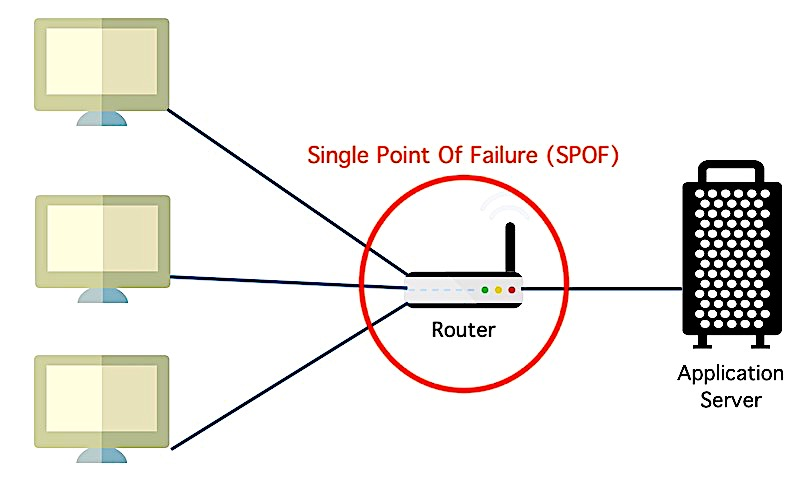
\includegraphics[width=10cm]{spof.jpg}
\caption{Exemplo de um \ac{SPOF}}
\end{figure}